as well\chapter{Related Work}
\label{relatedwork}
There has been a lot of research in the field of Virtual Reality and manipulation in a Virtual Environment (VE) which was most recent summarized by Jankowski in 2015\cite{interactions:Jankowski2015}. Further reading about specific techniques and tools can be found in Section \ref{theory:toolsandtech}. There have been a number of studies and implementations of systems that manipulates 3D environments using a HMD. The first major stride within this was in a study Butterworth in 1992 where a 3D surface modeling program was developed\cite{relatedwork:Butterworth1992}. This system was created using the same principles as CAD\footnote{http://www.autodesk.com/solutions/3d-cad-software} and similar software withing 3D object creation and manipulation. Since then there has been numerous other studies and applications within 3D object creation with a HMD\cite{relatedwork:bowman1996conceptual} \cite{relatedwork:moshell1995research} \cite{relatedwork:liang1994jdcad}.

Apart from the objects themselves, there has been some studies about using a HMD to manipulate 3D objects in relation to a VE. This approach is not as focused on 3D modelling as much as positioning and scaling of pre-fabricated objects in a 3D environment. In a study by Stoakley in 1995 a system called World in Miniature (WIM) was created\cite{relatedwork:stoakley1995virtual}. The premise of this system is to display a miniature version of the VE as well as the full-scale one. This allows the user to perform delicate manipulations at full scale, and bigger more fundamental changes on the miniature version. The user is holding a clipboard in one hand which represents the miniature world, and a interactive ball in the other for selecting and manipulating in 3D space. The same year, Mine introduced the "Immersive Simulation
Animation And Construction" system (ISAAC)\cite{relatedwork:mine1995isaac}. This system is primarily for designed for scene composition and interactive construction of virtual worlds. It tries to take advantage of the possibilities in the virtual world but keep the interaction scheme similar to the real world for easier adaptation to less experienced users. ISAAC uses multiple types of tools for object manipulation, such as ray-cast and direct manipulation (see Section \ref{theory:toolsandtech}) and multiple tools for the user to travel. This system is a showcase more then a application for real-world usage, as it demonstrates many of the possibilities with object and scene manipulation using a HMD but does not limit interaction tools based on a specific purpose or target-group. A concept with an intended purpose and demographic in mind was however presented by Deering, again in 1995\cite{relatedwork:deering1995holosketch}. The tool, HoloSketch, was created as a "what you see is what you get" virtual reality concept for real-time creation and manipulation of 3D objects and assemblies. It is designed for users with little to no programming knowledge to be able to create complex 3D objects and simple animations of an object. The display unit is based on the Virtual Holographic Workstation\cite{relatedwork:deering1992high}, which uses an external CRT monitor and head-tracked field sequential stereo shutter glasses. The virtual objects are manipulated with a 6 DOF wand/controller. The main user interface (UI) is a circular menu with diagonal lines to separate the different options(pie-menu), visualized in Figure \ref{fig:relatedwork:piemenu}. This UI is visible upon a button-press which hides the VE and displays the menu. This tool is specific with a purpose which is on the objects themselves, and not an entire experience or application environment.

\begin{figure}
  \centering
  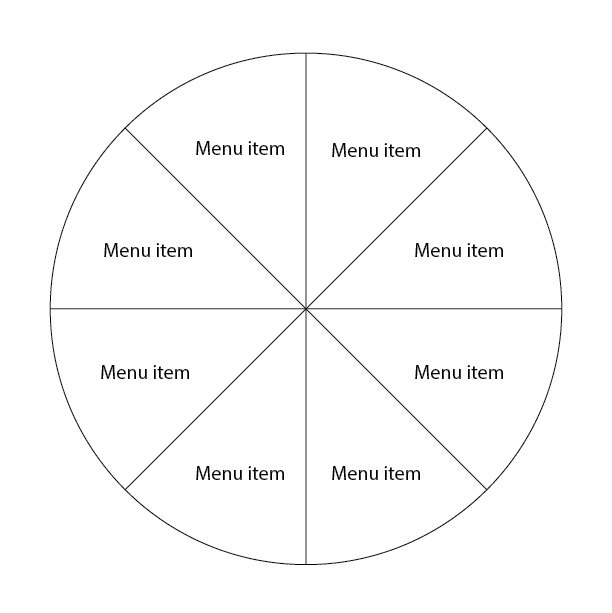
\includegraphics[width=.8\linewidth]{pie_menu.png}
\caption{Digital representation of a pie menu}
\label{fig:relatedwork:piemenu}
\end{figure}

There have been some studies about merging a regular workstation for 3D manipulation with a HMD\cite{UX:Alger2015}\cite{relatedwork:kijimaand1997transition}. Bowman et al. researched and developed with an objective similar to the objective of this thesis back in 1997\cite{relatedwork:kijimaand1997transition}. The authors investigated how to combine a regular work setup for 3D development with a HMD to remove the repeated transition between the two. Their Augmented Reality (AR) system is based on a real workstation which consists of a computer together with screen, keyboard and mouse. This is combined with a Projective Head Display (PHMD) to create an environment where the user can see projected 3D objects and still be able to use the workstation as usual.

This study will combine these previous findings and concretize how to usage of these tools can be adapted to the VR hardware available today for experience design projects.
